\chapter{Introduction}
\label{cha:intro}

This chapter describes a high level view of the SpiNNaker architecture and its main uses. It highlights also the motivation and aims of my project and how it may impact on the improvement of a large scale international research.

\section{Background}
\label{sec:background}

"SpiNNaker is a biologically inspired, massively parallel computing engine designed to facilitate the modelling and simulation of large-scale spiking neural networks of up to a billion neurons and trillion synapses (inter-neuron connections) in biological real time."\cite{painkras} Spinnaker was designed at the University of Manchester within an EPSRC-funded project in collaboration with other institutions.XXX

The Spinnaker research, funded by the Human Brain Project (HBP)[definition] started on XXX 2005? XXX and has the XX final aim? XX of simulating the human brain.

\section{Project Aim}
\label{sec:aim}


-evaluate how efficient Spinnaker is with a general purpose application.
-test usability -- im a user! 

This research project involves making use of the emerging SpiNNaker software stack and hardware infrastructure, both optimised for neural network simulations, in order to explore and evaluate its usability and performance as a general purpose platform. This has been achieved through the development of a distributed Key-Value store and a Relational Database Management System with limited scope.

SpiNNaker is particularly strong at parallel execution at low power consumption, which appealed as an extraordinary opportunity to store data in a distributed way, under a database management system. This would ideally allow a linear speedup of data retrival in comparison with a sequential system.

This project has grown to be the largest non-neuromorphic application now available as part of the SpiNNaker API.

In addition to usability testing, performance benchmarks have been gathered for this application, allowing analysis which can provide insights for improvements to the current architecture, possibly influencing on changes to reflect on the next generation of the chip: SpiNNaker 2. A 

aim: balance of memory and processing power on the chip, etc.

\section{SpiNNaker Architecture}

%https://www.arm.com/products/processors/classic/arm9/arm968.php
The custom built SpiNNaker chips each contain 18 ARM968 (word aligned, 32-bit arch, 600-MHz?) processing cores sharing 128-MB of in-chip dynamic memory (SDRAM). Following the Harvard Architecture[...], each core in the chip holds a private 32-KB instruction memory and 64-KB data memory.

explain host computer, etc..

\begin{figure}
\begin{center}
	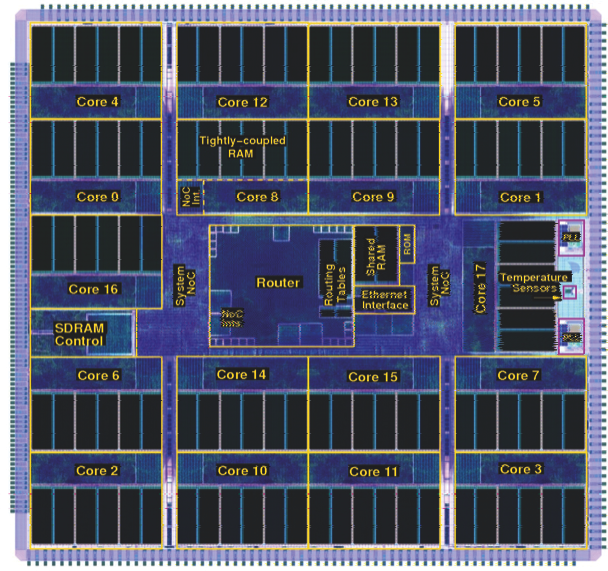
\includegraphics[width=0.7\textwidth, natwidth=608, natheight=571]{images/chip.png}
\end{center}
\caption{SpiNNaker chip layout}
\end{figure}

There are currently two types of SpiNNaker boards:
\begin{itemize}
\item SpiNN-3, composed of 4 chips, thus a total of 72 processing cores
\item SpiNN-4, composed of 48 chips, this a total of 864 processing cores
\end{itemize}

A standard Spinnaker board is composed of 48 descentralised, power efficient, Spinnaker chip multiprocessor (CMP) dies, each containing 18 ARM968 processing cores sharing 128-MB of in-chip dynamic memory (SDRAM). In a standard environment each ARM models up to 1000 neurons, which can communicate to each other through atomic 'spike' events using the on- and inter-chip communication fabric.\cite{datasheet}

event driven architecture
donught shaped

\begin{figure}
\centering
\begin{minipage}{.5\textwidth}
  \centering
  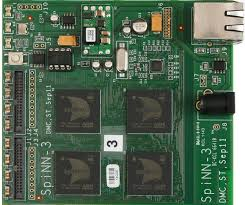
\includegraphics[width=0.4\linewidth, natwidth=245, natheight=205]{images/4node.jpg}
  \captionof{figure}{SpiNN-3}
  \label{fig:4node}
\end{minipage}%
\begin{minipage}{.5\textwidth}
  \centering
  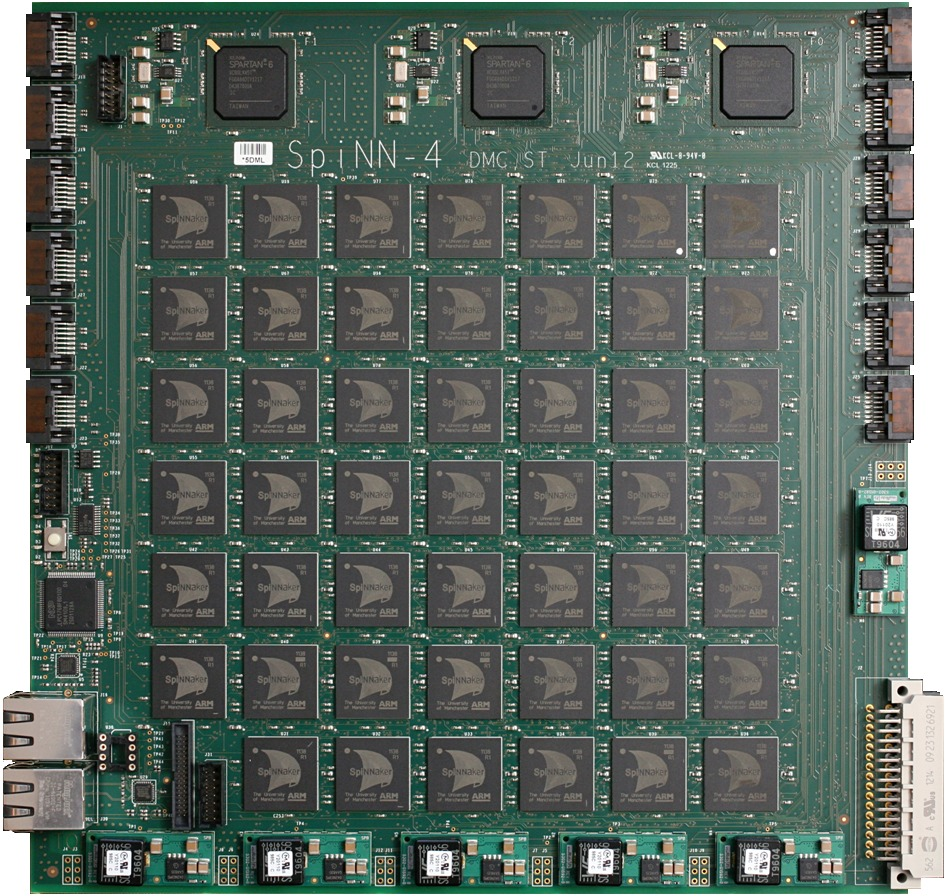
\includegraphics[width=0.9\linewidth, natwidth=945, natheight=896]{images/48node.jpg}
  \captionof{figure}{SpiNN-4}
  \label{fig:48node}
\end{minipage}
\end{figure}

\subsection{SpiNNaker Communication fabric}

XXXX should this be on the introduction???
event driven

The SpiNNaker API allows the utilisation of 4 different communication protocols between cores in the system. These packets trigger prioratised interrupts on the receiver, as it is an event driven architecture. These can be used to spread work load and transmit information initially private to a core.
It is worth noting that \textbf{none of these protocols guarantee successful delivery of data} and this effect is worsen if there is large traffic in the communication fabric. This means sending a large amount of packets symultaneously will result on packet drops.

\begin{itemize}
\item \textbf{Multicast (MC)}
The MC protocol, originally designed to simulate neural spikes, predicts a sigle source core casting a packet to multiple destinations. The packet contains only a 32 bit routing key, used by an external process to carry out the delivery, and an optional 32 bit payload, both provided at the source.

router.. routing table
\item \textbf{Point to Point (P2P)}
XXX
On top of the P2P layer, the SpiNNaker Datagram Protocol (SDP) was developed (build/written?) to allow larger transfers of data, of up to 280 (?) bytes, to reduce queueing on receival... (find the paper...)
%https://spinnaker.cs.man.ac.uk/tiki-download_wiki_attachment.php?attId=16

Using SDP, the SpiNNaker API XXX a User Datagram Protocol (UDP), allowing a two-way communication over IP addresses with the host machine. This allows uploading binaries and communicating back and forth with the hardware.

unreliability....
unreliable spikes (see that guy's paper...)

\item \textbf{Nearest-neighbour (NN)}
\item \textbf{Fixed-route (FR)}
\end{itemize}

[spinnaker datasheet page 30]

-mention DTCM only 64kb (so preferred to use SDRAM)
-look at your logbook for query plan stuff (at the start)
-debugging with ybug. testing with unit tests
-supported operations
-host is stateless
-tested on real data?

Each processor node on SpiNNaker includes a communication controller which is responsible for generating and receiving packets to and from the communication network.
The SpiNNaker architecture offers a range of...
all of which are unreliable!!

packet formats:


